
\section{Introduction}
\label{sec:intro}
\iffalse
TODO:
\begin{itemize}
    \item Explicar el problema. Soluciones propuestas hasta ahora. Por qué no son suficientes. En qué consiste la nuestra.
    \item Definición general aplicación propuesta. Validez para PoS card fraud or internet frauds (CNP: Card Not Present frauds)... pero que hemos concretado en el caso de los ATM fraud.
    \fmc{Poner aquí contexto sobre los distintos tipos de fraude y sus estadísticas: referencia al informe SEPA ("Seventh report on card fraud typos")}
    \item Explicar cómo está organizado el documento.
\end{itemize}
\fi

As an example of critical decision making scenario in real time, we consider 
the problem of detecting anomalous usage patterns in bank card transactions. 
In particular, suppose a card is used to withdraw money in two different locations 
in an elapsed time interval that makes it impossible for the cardholder to physically 
move from one location to the other; let us suppose, for instance, 
that one ATM is in Barcelona and the other in Madrid and two transactions are made with 
the same card in less than an hour, one at each ATM. 
Note that we are not concerned here with the typical physical sabotage of ATMs to steal/clone data, 
but instead we are concerned with possible criminal situations beyond sabotage, 
such as cloned bank cards. While using a cloned bank card chances are that  
suspicious patterns like the one described above arise. 
This is exactly what our proposal aims to detect in order to prevent a crime from being carried out, 
thereby protecting the interests of both, the bank and the cardholder.\\

Although from a classical point of view databases consider data as persistent~\cite{abiteboul1995foundations}, 
nowadays this perspective is changing~\cite{babu2001continuous,zaniolo2012logical} as data is in motion, continuously changing 
and (possibly) unlimited. 
This is the case of ATM transactions. Indeed, transactions occur continuously and are not
(necessarily) bounded. 
In this setting, the fact that transactions should be somehow represented in banking 
databases makes us reconsider the meaning of their persistence in banking systems 
raising the following two questions: 
(i) What is the appropriate data model to deal with this kind of transactions? 
and (ii) What is the appropriate query model?\\

\noindent
Regarding the data model, the new nature of data requires a \emph{de facto} 
new database paradigm -\emph{continuously evolving  databases}- 
where data can be both \emph{stable} and \emph{volatile}. 
Even though evolving databases can be implemented according to any approach, 
graph databases seem especially well suited here {\cite{GDB-angles2008survey, GDB-kumar2015graph}. 
Indeed, the natural way to process evolving graphs as streams of edges gives insights 
on how to proceed in order to maintain dynamic graph databases.  
Hence, we consider that a suitable data model is a \emph{continuously evolving data graph}, 
a graph having persistent (\emph{stable}) as well as non persistent (\emph{volatile}) relations. 
Stable relations correspond to edges occurring in standard graph databases while volatile relations 
are edges arriving in data streams during a set time interval. 
Once this time interval is over, the relations are no longer valid so that there is no need to store 
them in the (stable) graph database. 
Volatile relations induce subgraphs that exist only while the relations are still valid. 
%
\noindent
In this work we tackled the problem of evaluating continuous queries corresponding to 
\emph{anomalous patterns} of ATM transactions against a continuously evolving graph database  
representing a bank database.\\

Without loss of generality we use  \emph{Property Graphs} (PG) 
\cite{PG-angles2017foundations, angles2018propertyGraphDatabaseModel} 
as the basic reference graph data model. 
As an example, Figure \ref{fig:constinuousPGa} depicts part of a schema of a 
PG database where stable relations correspond to the data that a bank 
typically gathers on its issued cards, ATMs (Automated Teller Machines) network, etc. 
Volatile relations model the interaction between cards and ATM entities.\\
%
\begin{figure*}[h]
    \centering
    \begin{subfigure}[b]{0.6\textwidth}
        \centering
        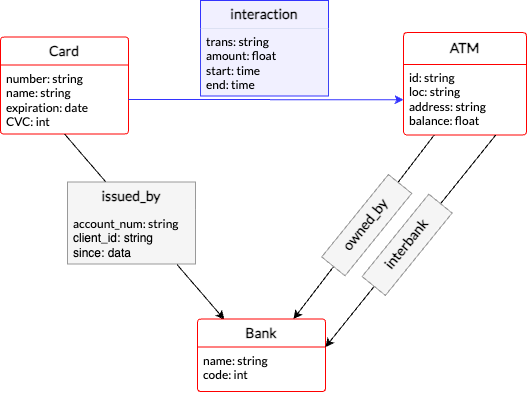
\includegraphics[width=0.85\textwidth]{images/schema.png}
        \caption{Part of a schema of a PG}
         \label{fig:constinuousPGa}
    \end{subfigure}%
     ~ 
    \begin{subfigure}[b]{0.4\textwidth}
        \centering
        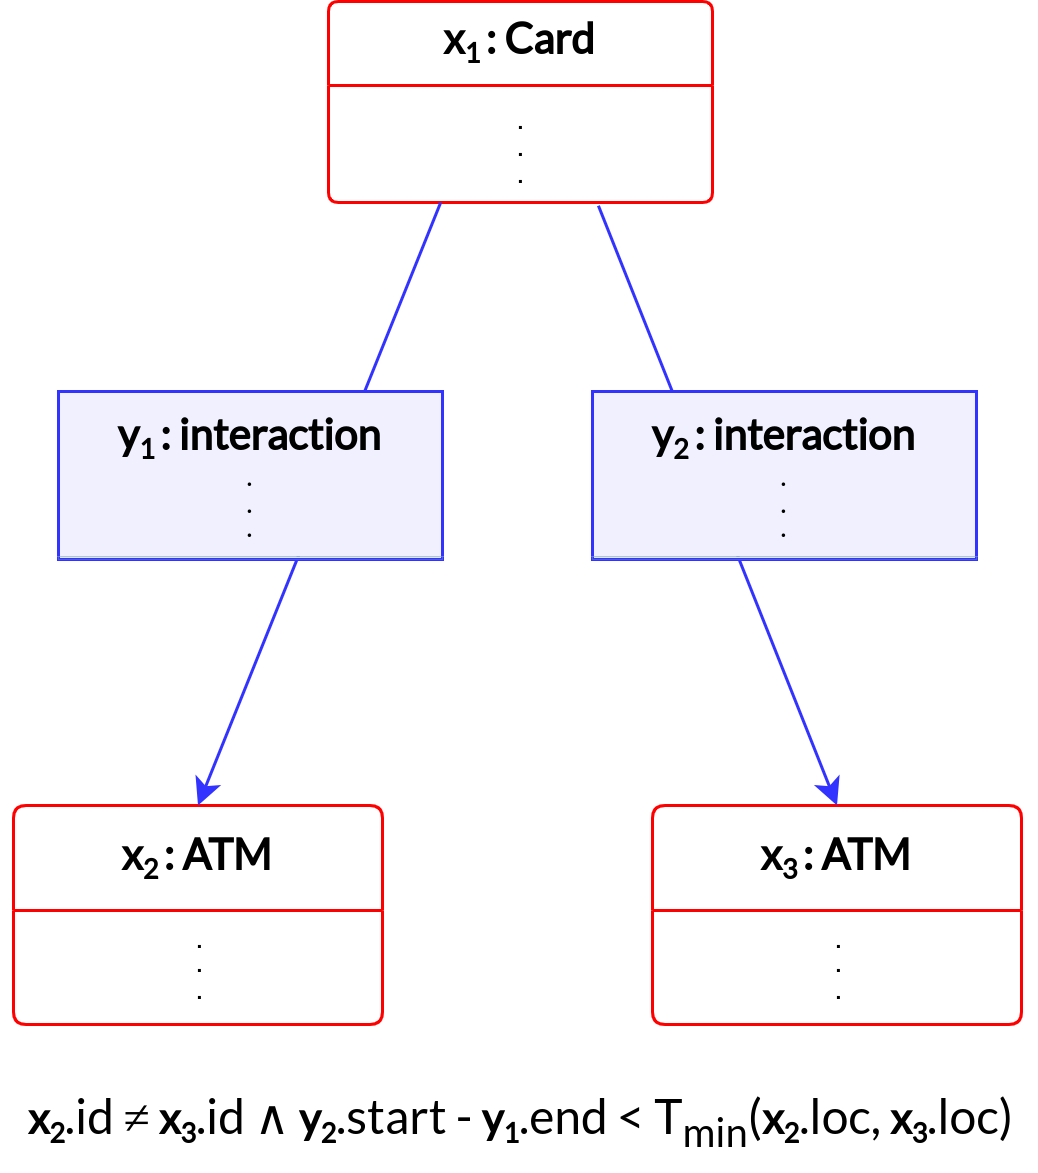
\includegraphics[width=0.85\textwidth]{images/graphPattern.png}
        \caption{Pattern of anomalous transactions}
        \label{fig:constinuousPGb}
    \end{subfigure}
    \caption{Part of a PG schema specifying volatile (\textsf{interaction} edges) and stable  (\textsf{issued\_by, owned\_by, interbank} edges) relations in an evolving ATM Network and a continuous query pattern.}
    \label{fig:constinuousPG}
\end{figure*}
%

\noindent
Concerning the query model, fixed queries evaluated over data streams are known 
as \emph{continuous queries} \cite{CQ-babu2001continuous,CQ-zaniolo2012logical}. 
Thus, instead of classical query evaluation processes we envision \emph{incremental/progressive} 
query evaluation processes. 
A query on a PG database can be seen as a PG graph pattern with 
constraints over some of its properties. 
Evaluating such a query consists on identifying if there is a 
subgraph of the database that matches 
the given pattern and satisfies its constraints. 
Figure \ref{fig:constinuousPGb} depicts the pattern 
corresponding to an anomalous situation in 
the volatile (PG) subgraph of the considered database. 
This is, a constrained graph pattern corresponding to a continuous query. 
An  anomalous pattern of ATM transactions must be identified in 
the volatile (PG) subgraph of the considered database.\\

The problem of progressively identifying and enumerating bitriangles 
(i.e. a specific graph pattern) 
in bipartite evolving graphs using the 
\emph{Dynamic Pipeline Approach} (DPA)\cite{DP-pasarella2024computational} 
have been successfully solved by Royo-Sales \cite{DP-bitriangles2021}.  
Let us observe that the problem of evaluating continuous queries over 
\emph{continuously evolving PGs} 
belongs to the same family of problems and hence we propose to address 
it using the same stream 
processing computational model.
%the {Dynamic Pipeline Approach}\cite{DP-pasarella2024computational}.  
Figure \ref{fig:theProblem} illustrates the model associated to the problem described at 
the beginning of this section. 
%
\begin{figure}[h]
         \centering
         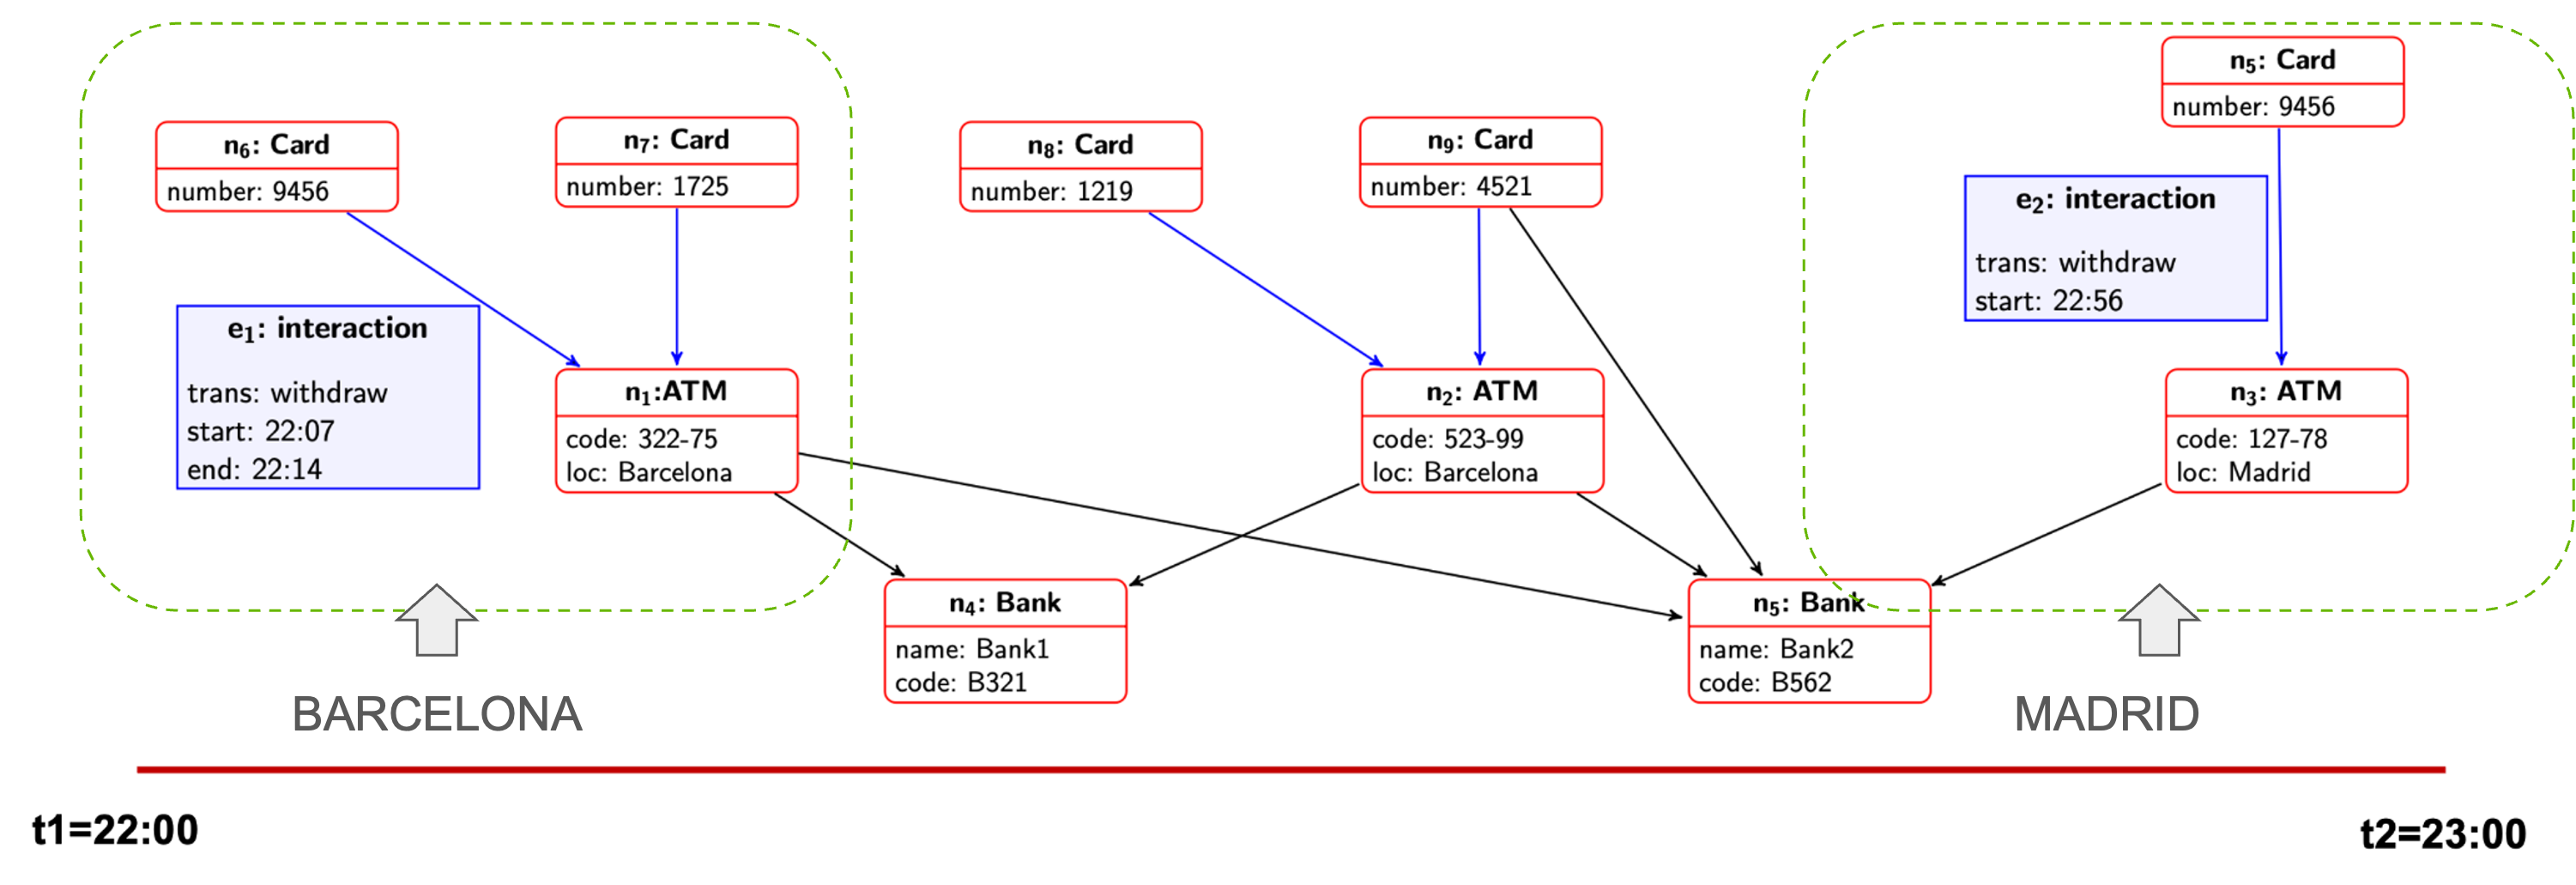
\includegraphics[width=0.85\textwidth]{images/theProblem.png}
         \caption{Example of the occurrence of anomalous ATM transactions in (a part of) 
         a continuously evolving PG over a time interval: the card \textsf{9456} is used twice at ATMs 
         in different cities, within one hour. 
         However, to get from one of the cities to the other and vice versa requires more 
         than one hour using any means of transport. 
         This example could represent a possible 
         crime pattern after a case of \emph{skimming} and \emph{cloning}.}
         \label{fig:theProblem}
\end{figure}
%
In addition to identify the query pattern, the constraint satisfaction 
over properties must be checked also.  
The evaluation process, done by a \emph{Continuous Query Engine} (CQE) 
is based on the dynamic pipeline computational 
model \cite{DP-pasarella2024computational} and  
emits  answers (alarms) as soon as anomalous patterns are identified. 
Moreover, in a real application,  
when required -as for further legal or auditing purposes- 
timestamped occurrences of volatile relations can  be kept in a log file. 
Figure \ref{fig:DP_ATM} depicts a basic architecture of a CQE.
%
\begin{figure}[h]
         \centering
         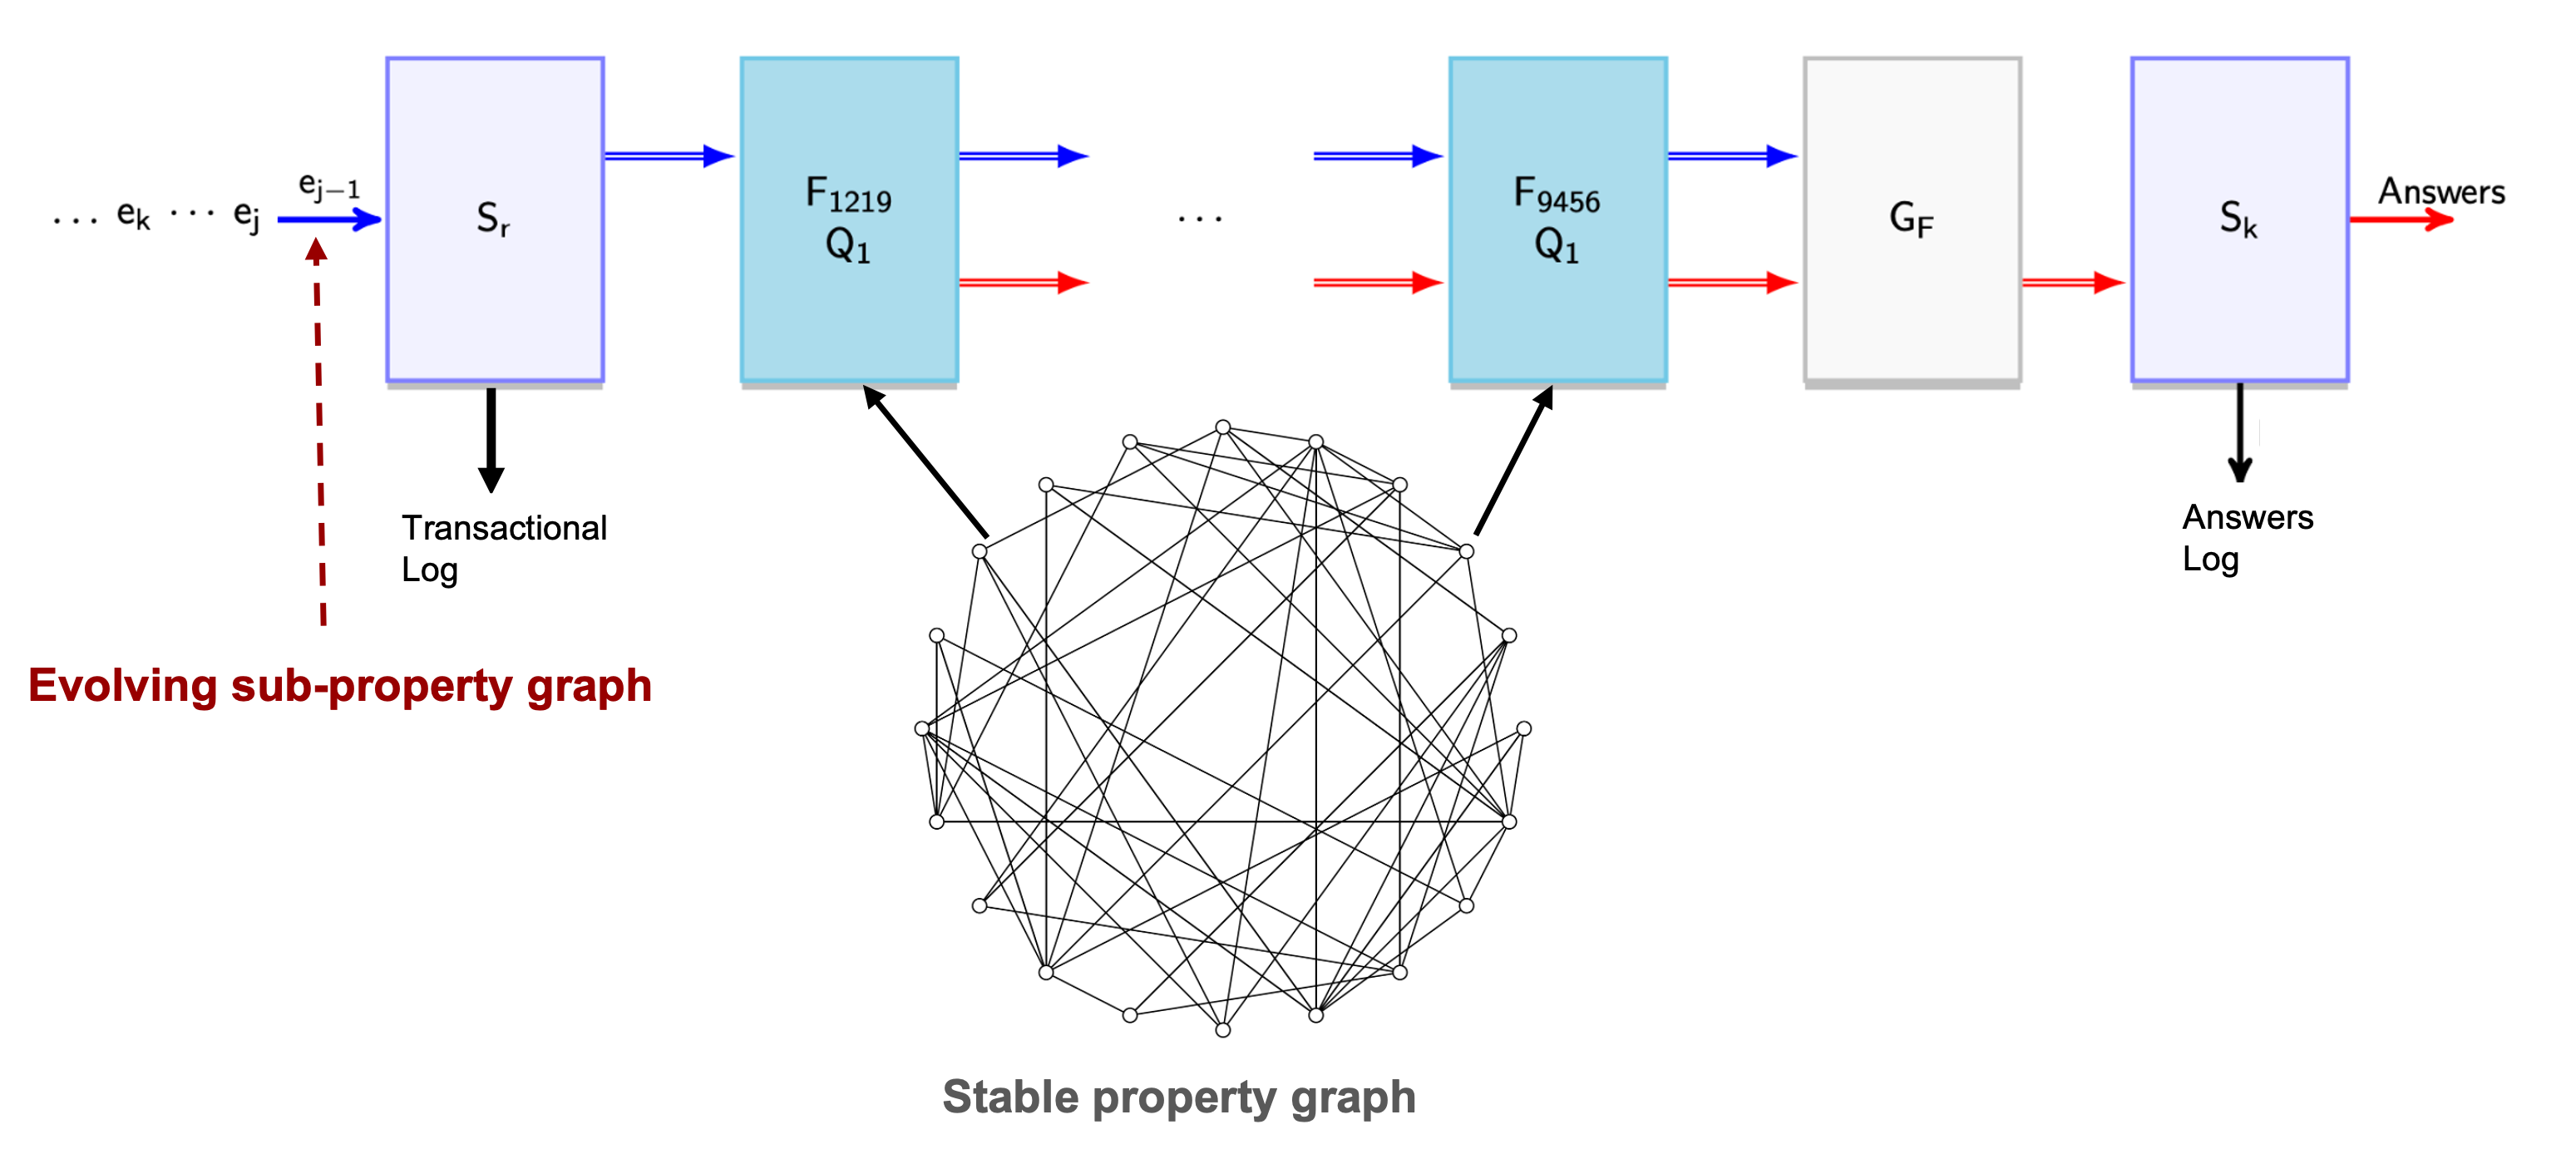
\includegraphics[width=0.7\textwidth]{images/architecture.png}
         \caption{Preliminary continuous query engine architecture for detecting anomalous 
         ATM transactions based on the dynamic pipeline computational model. 
         Considering the schema given in Figure \ref{fig:constinuousPGa}, 
         in this directed (multi) graph presentation of the $\mathsf{DP_{ATM}}$, 
         the arriving input data is a stream  $\mathsf{\langle \dots e_k\dots e_j \: e_{j-1}\rangle}$ 
         corresponding to \textsf{interactions} (volatile relations). 
         Boxes (vertices) represent \emph{stateful} processes called \emph{stages} 
         and internal arrows in the pipeline represent channels. 
         Blue channels carry interaction edges and red channels carry detected anomalies (answers).  
         $\mathsf{S_r}$ and $\mathsf{S_k}$ correspond to the \textsf{Source} and \textsf{Sink} 
         stages which receive input data and results, respectively. 
         \textsf{Filter} stages, $\mathsf{F_{N}}$, are parameterized with the value of the property 
         \textsf{number} ($\mathsf{N}$) of \textsf{Card} vertices. 
         The \textsf{Generator} stage, $\mathsf{G_F}$, is in charge of spawning new filters, 
         when required. The stable PG is a standard bank database (i.e. without volatile relations). 
         Transactional log and Answers log keep input interactions and answers, respectively.
         }
         \label{fig:DP_ATM}
\end{figure}

In order to test the practical suitability of our proposal, 
we have implemented it in the \texttt{Go} programming 
language since this language easily provides connection 
to existing implementations of Neo4j graph databases 
such as the one we use in this work, in addition to providing the necessary 
tools to exploit the parallel 
and distributed properties of the DPA with which we represent our proposal.
Additionally, in order to experiment with the performance of our model, 
we provide a program capable of generating synthetic datasets useful 
to simulate bank graph databases including several parameters such as the users, 
their card holders, their ATMs geographically distributed, 
the stream of transactions, etc.\cite{ATM-DP-github}
We assessed our model with two different bank sizes considering standard metrics as well as specific ones \cite{exps-diefficiency} for measuring continuous behavior  
and we could observe that (compared to a sequentially implemented system) 
the proposal using the DPA performs clearly better, 
providing almost immediate responses to the tested queries. 
Additionally, as opposed to artificial intelligence approaches \cite{ahmed2016survey,} to predict frauds, 
ours provides 100\% of effectiveness detecting fraud patterns. 
This is, there is no place to consider false alarms (false positive recognition of pattern)  
or ignore alarms due to non-recognition of patterns (false negative) since,  
in presence of the studied fraud pattern, the CQE will recognize it. Partial results of this work were reported and presented in the Alberto Mendelzon Workshop 2024 \cite{martincanfran2024AMW}. 
We can summarize the contributions of this work as follows.

\paragraph{Contributions.}
\begin{itemize}
\item A general technique for addressing the problem of continuous 
query evaluation against an evolving graph database by decomposing 
the data graph into \emph{volatile} and \emph{stable} well defined subgraphs, 
using a stream processing approach.  
Among the advantages of using the dynamic pipeline computational 
model are its parallel/concurrent nature and its suitability for 
developing real-time systems that emit results as they are computed, 
in a progressive way. 
\item A characterization of some possible fraud graph patterns. Even non-exhaustive, to our knowledge, it is a first specification of what must be consider a fraud pattern in terms of (continuous) graph databases. This characterization is useful not only when considering ATM transactions but, in general,  for any bank cards online transactions.
\item A continuous query engine  to detect abnormal or suspicious ATM transactions. 
To our knowledge, most of the work addressing this topic provide a delayed 
detection based on predictions given by ML systems. 
Also, it is frequent the classical treatment of the problem by consulting 
log files because of the complaint of customers when detecting by 
themselves some weird  movement in their accounts. 
This involves annoying processes for customers in order to have their money back. 
The idea is that, in presence of some weird  finding in an ATM transaction, 
banks have a tool able to either ask card holders for authorizations 
or to take any action preventing other fraud at real-time.
\item Given the sensitive nature of banking data and transactions, 
there are no repositories that offer this type of datasets for empirical studies. 
In this work, we have created an open synthetic repository for this purpose. 
\end{itemize}

The rest of this work is organized as follows. 
In Section \ref{sec:related_work}, we describe the related existing work while, 
in Section \ref{sec:prelim}, we give the required preliminaries to follow the whole work 
regarding graph databases, graph fraud patterns, the dynamic pipeline paradigm and
the metrics used to evaluate the features of our proposal.
In Section \ref{sec:proposal}, we describe the details of our proposal by 
defining anomalous patterns of transactions, how to 
model and implement the continuous query engine, the used data model and query model 
as well as the architecture of the continuous query engine.
Section \ref{sec:CQE-DPATM} is devoted to the continuous query engine, the 
$\mathsf{DP_{ATM}}$. The experiments are described in Section \ref{sec:experiments} where 
the different evaluation scenarios, the experimental settings, the datasets and 
the stream configurations are considered. The experimental results are analyzed in Section \ref{sec:results}
and in Section \ref{sec:concl} we give some conclusions and proposals for further work.
